\documentclass[UTF8]{ctexart}
\usepackage{lmodern}
\usepackage{amsmath}
\usepackage{graphicx}
\usepackage{float}%提供float浮动环境
\usepackage{booktabs}%提供命令\toprule、\midrule、\bottomrule
\usepackage{geometry}

\geometry{a4paper,left=2cm,right=2cm,top=2cm,bottom=2cm}

\title{{电子技术基础实验} \\ \textbf{实验五\ 阻抗变换器与混沌电路}}
\author{\\\textbf{祝尔乐}
        \\\textbf{未央-电01}
        }
\date{\textbf{\today}}

\begin{document}
\maketitle

\section*{一.实验目的}

\subsection*{1、熟悉运算放电器工作原理}
\subsection*{2、了解由运算放大器构成的阻抗变换器}
\subsection*{3、了解电子电路中的混沌现象}
\subsection*{4、熟悉电路仿真与调试}

\section*{二.实验内容}

\subsection*{1.蔡氏混沌电路}

\begin{figure}[H]
        \centering
        \includegraphics*[width = 0.5\textwidth]{1-电路图.png}
        \caption{电路图1}
\end{figure}

按照电路图1连接电路。

\subsubsection*{(1)调节 $R_1$,测量 $v_1$ 和 $v_2$ 波形,观察当 $R_1$约在 1.7kΩ 上下时的波形变化,
并与仿真结果比较}

先进行电路仿真,
\begin{figure}[H]
        \centering
        \includegraphics*[width = 0.5\textwidth]{1-1-1.7k.jpg}
        \caption{$R_1 = 1.7k\Omega$}
\end{figure}
\begin{figure}[H]
        \centering
        \includegraphics*[width = 0.5\textwidth]{1-1-1.75k.jpg}
        \caption{$R_1 = 1.75k\Omega$}
\end{figure}
\begin{figure}[H]
        \centering
        \includegraphics*[width = 0.5\textwidth]{1-1-1.65k.jpg}
        \caption{$R_1 = 1.65k\Omega$}
\end{figure}

按照电路图搭建电路,将电路调节为$R1=1.7k \Omega$,
得到电路波形为:

\begin{figure}[H]
        \centering
        \includegraphics*[width = 0.5\textwidth]{1-1-1.7k-r.jpg}
        \caption{$R_1 = 1.7k \Omega$}
\end{figure}

可以看出波形比较规则,无法产生混沌。

我们调节可变电阻器,使其阻值变小,看到波形出现比较理想的情况:

\begin{figure}[H]
        \centering
        \includegraphics*[width = 0.5\textwidth]{1-1-adjust-r.jpg}
        \caption{$R_1$调节后}
\end{figure}


\subsubsection*{(2)用示波器 XY 显示模式(Utility->显示->格式->XY),调节 $R_1$ 阻值
(1.6/1.7/1.8 kΩ),测量 $v_1$ 与 $v_2$ 的波形图,并与仿真结果比较。}

先对电路进行仿真,仿真结果如下:
\begin{figure}[H]
        \centering
        \includegraphics*[width = 0.5\textwidth]{1-2-1.7k.jpg}
        \caption{$R_1 = 1.7k\Omega$}
\end{figure}
\begin{figure}[H]
        \centering
        \includegraphics*[width = 0.5\textwidth]{1-2-1.75k.jpg}
        \caption{$R_1 = 1.75k\Omega$}
\end{figure}
\begin{figure}[H]
        \centering
        \includegraphics*[width = 0.5\textwidth]{1-2-1.65k.jpg}
        \caption{$R_1 = 1.65k\Omega$}
\end{figure}

实际测量时,我们调整$R_1$的阻值在$1.6k \Omega$左右,观察v1-v2的波形,波形如下图:

\begin{figure}[H]
        \centering
        \includegraphics*[width = 0.5\textwidth]{1-2-1.61k-r.jpg}
        \caption{$R_1 = 1.61k\Omega$}
\end{figure}
\begin{figure}[H]
        \centering
        \includegraphics*[width = 0.5\textwidth]{1-2-1.58k-r.jpg}
        \caption{$R_1 = 1.58k\Omega$}
\end{figure}

\subsubsection*{(3)分析虚线框中运放电路的功能,及其在整个电路中所起的作用。}

本题电路为蔡氏混沌电路,产生混沌的基本条件为:

1.一个或者多个的非线性元件
2.一个或者多个的本地有源电阻
3.三个或者更多个能量存储元件

题目中两个电容和电感作为能量储存元件,可变电阻器作为本地有源电阻,
而虚线框中的运算放大器可作为非线性元件使用。

\subsection*{2.等效电感}

\begin{figure}[H]
        \centering
        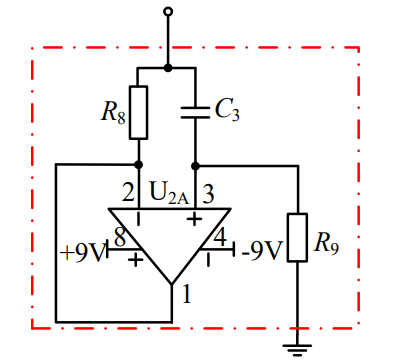
\includegraphics[width = 0.4\textwidth]{2-电路图.png}
        \caption{2-电路图}
\end{figure}

电路参数:$R_8 = ~15\Omega, R_9=100k \Omega, C_3=10nF$。

\subsubsection*{(1)分析电路功能}

运算放大器正极接了一个微分电路,负极直接与输出相连,深度负反馈,
由虚短虚断可知,电路此时相当于一个电感(对电流进行微分)。


\subsubsection*{(2)尝试用图 2 所示电路代替图 1 中的电感 L,完成任务 1(2)。}

对电路进行仿真,仿真结果如下:
\begin{figure}[H]
        \centering
        \includegraphics*[width = 0.5\textwidth]{2-2-1.7k.jpg}
        \caption{$R_1 = 1.7k\Omega$}
\end{figure}
\begin{figure}[H]
        \centering
        \includegraphics*[width = 0.5\textwidth]{2-2-1.75k.jpg}
        \caption{$R_1 = 1.75k\Omega$}
\end{figure}
\begin{figure}[H]
        \centering
        \includegraphics*[width = 0.5\textwidth]{2-2-1.65k.jpg}
        \caption{$R_1 = 1.65k\Omega$}
\end{figure}

实际搭建电路,得到波形图:

\begin{figure}[H]
        \centering
        \includegraphics*[width = 0.5\textwidth]{2-2-1-r.jpg}
        \caption{$R_1 = 1.66k\Omega$}
\end{figure}
\begin{figure}[H]
        \centering
        \includegraphics*[width = 0.5\textwidth]{2-2-2-r.jpg}
        \caption{$R_1 = 1.71k\Omega$}
\end{figure}

由波形图可以看出,电路2起到了电感的作用,也可以产生蔡氏混沌。

\section*{参考资料}

http://staff.ustc.edu.cn/~bjye/em/student/2019S/2019S-02-10.pdf

\end{document}